\documentclass[11pt,letterpaper]{article} % for a short document

% Bibliography
\usepackage[authordate,strict,autolang=hyphen,bibencoding=inputenc,doi=true,isbn=false,annotation=false]{biblatex-chicago}
\usepackage{graphicx}
\DeclareGraphicsExtensions{.pdf,.png,.jpg}
\usepackage[section]{placeins}
\addbibresource{../references/references.bib}
\usepackage{booktabs}
\usepackage[affil-it]{authblk} % pretty author nameuse
\usepackage{verbatim} % mono spaced as needed
\usepackage{color} % for PMH's comments
\usepackage{soul} % for strikethrough

% italicize 'et al.'
\renewbibmacro*{name:andothers}{% Based on name:andothers from biblatex.def
  \ifboolexpr{
    test {\ifnumequal{\value{listcount}}{\value{liststop}}}
    and
    test \ifmorenames
  }
    {\ifnumgreater{\value{liststop}}{1}
       {\finalandcomma}
       {}%
     \andothersdelim\bibstring[\emph]{andothers}}
    {}}

%---------------------------------------- title, author, date
\title{Reproducible sausage network buffers for built environment measurement: an open source GIS approach}
% \author[*]{Philip M. Hurvitz}
% \author[*]{}
% \author[*]{Eric J. Howard}
\author{Philip M. Hurvitz%
  \thanks{Electronic address: \texttt{phurvitz@uw.edu.edu}; Corresponding author}}

\author{Peter Schmiedeskamp%
  \thanks{Electronic address: \texttt{pschmied@uw.edu}}}

\author{Eric J. Howard%
  \thanks{Electronic address: \texttt{ejhoward@uw.edu}}}
  
\affil{Department of Urban Design and Planning, University of Washington}

\date{}

%----------------------------------------
%%% BEGIN DOCUMENT

\begin{document}

\maketitle

\section*{Background}
Associations between built environment exposures and behaviors or health outcomes are of great interest in public health research. Geographic Information Systems (GIS) methods for quantifying exposure to features within the built environment have developed rapidly, from census-unit approaches \parencite{Morland2002a}, to Euclidan (`circular' or `crow-flies') buffers around geocoded home locations \parencite{Moudon2002}, to network-distance buffers \parencite{Frank2005}. Buffer measures have become preferred because they capture only those features near to specific locations and avoid the Modifiable Areal Unit Problem \parencite{Openshaw1984}, with network buffers favored due to their ability to mask out areas that are reasonably inaccessible by foot or vehicle \parencite{Oliver2007}. 

\textcite{Forsyth2014sausage}
identified a threat to replicability for studies using such
network-based buffers, due to changes in how Esri's
market-leading GIS software has calculated them across different software versions. In response,
the authors proposed ``sausage'' network buffers,
created via a transparent algorithm, for use in measuring aspects of
urban form related to food and physical activity. The algorithm was operationalized using Esri's ArcGIS desktop GIS software on Microsoft Windows, but owing to its simplicity and transparency, was described as potentially 
replicable and cross-platform. Their paper called on others to validate sausage buffers
created using other GIS software on other platforms. 

This paper serves several purposes. It answers \citeauthor{Forsyth2014sausage}'s call by presenting and validating an alternate method for the creation of sausage buffers using readily available, cross-platform, free and open source software; in doing so it also introduces and demonstrates the specific software used for development of the method, PostGIS \parencite{ThePostGISDevelopmentGroup2008}, as an alternative to proprietary, commercial GIS software. PostGIS is an extension to the free and open source relational database PostgreSQL \parencite{ThePostgreSQLGlobalDevelopmentGroup2008}. In this paper we focus on the use of network and buffer analysis, but PostGIS contains a large set of geoprocessing functions common to most desktop GIS applications, such as geometric overlay, coordinate projections, and raster analysis.

%Let's mention something about reproducibility up front.
The methods presented here are also in part a response to a growing
call from numerous disciplines to ensure computer aided
analyses are truly reproducible. The basic standard for reproducibility is
that the data used are made available, and that analyses are shared in the
form of computer code \parencite{Peng2011computational}. Notably, the
methods presented here are reproducible because the analyses are fully
automated using computer code, rather than being reliant on a set of
manual procedures. The code and the data have been made publicly
available, so that other researchers may both review and benefit from this work.\footnote{need to package up code and data, upload to UW's
  repository, and then see about generating a DOI.}  Further, building
these methods atop free and open source software achieves a higher
standard of reproducibility by eliminating dependencies on any ``black
box'' methods within proprietary software that may be necessary in data processing. In principle, this means that every piece of
software, as well as the specific analytic code and data used in these methods, is open to scrutiny.

% Relevance to planning and epidemiology
Developing geoprocessing methods around free and open source tools
holds particular benefits for disciplines such as epidemiology, public
policy, and urban planning because of the reduced barriers to adoption
for practitioners and advocates outside of larger institutions. Academic
institutions and larger public agencies may be able to afford costly software
applications. However, smaller agencies or advocacy groups wishing to
perform quantitative analysis of built environment might be unable to
make use of even transparently described analyses that are reliant on proprietary software, simply due to the
cost of software licensing fees.

% Not a literature review, per se. Since we are developing a methods
% paper largely in response to one particularly important method, I'm
% not sure how important a full-blown review is. Open to suggestions,
% however. This could potentially be split off and developed into
% something more complete. 
% PMH: I agree, we aren't doing an evaluation of the use of PostGIS in research.
Finally, the PostGIS platform is especially beneficial in that it
naturally facilitates reproducible, scripted analyses, as well as 
provides the core infrastructure for data storage and management on even very large research
projects. \textcite{hurvitz2014emerging} describe the use of
PostgreSQL/PostGIS to manage and process geospatial and timeseries
data from a variety of sources including Global Positioning Systems (GPS) and
accelerometers for very large data sets. We are admittedly neither first nor alone in identifying
PostGIS for use in research. A keyword search for ``PostGIS'' using
ISI Web of Science identified 35 \textcolor{red}{[I got 50 today!]} articles across a number of
disciplines describing the use of PostGIS in research. In the
transportation sector, \textcite{Wang2015routable} also used PostGIS
to store and analyze a large number of GPS traces in order to infer
characteristics about roadways such as position and rules, for the
purposes of generating routable roadway networks. In another recent
article, \textcite{Brovelli2015FOSS} describe the use of PostGIS
together with GeoServer to collect data about roadway pavement
conditions from the general public. Notable in that study is the
potential for PostGIS in supporting digitally-mediated public
participation. However, a PubMed search for ``PostGIS'' resulted in only one paper \parencite{Rowlingson2013}. In contrast, Web of Science and PubMed searches for ``ArcGIS'' resulted in 1,674 and 394 citations, respectively. This indicates that a number of researchers who could potentially benefit from the use of PostGIS may simply be unaware of its existence.


\section*{Methods}
% Set-up and software pgRouting 2.x on OpenBSD 5.7 i5
Following the process outlined in 
\textcite{Forsyth2014sausage} and described in step-by-step detail in \textcite{ Forsyth2012proto}, we implemented the
sausage buffering technique using PostgreSQL 
with PostGIS and the pgRouting \parencite{pgRoutingContributors2013} extension, which implements a number of network routing algorithms, including Dijkstra's shortest path \parencite{Dijkstra1959}, which is also used in the ArcGIS Network Analyst exension. Using that technique we
generated 200 sausage buffers around randomly selected points. We then
compared those results to buffers analogously created in ArcGIS Desktop
10.2.X, for use as a basis for comparison with the results presented
by \citeauthor{Forsyth2014sausage}. Table \ref{tab:software} lists
software versions used in this analysis.


\begin{table}[h!]
  \centering
  \caption{Software used to generate PostGIS and ArcGIS sausage buffers}
  \begin{tabular}{llr}
  \toprule
  Buffer type & Software & Version \\
  \midrule
PostGIS/pgRouting & OpenBSD (Operating System) & 5.7 \\
              & PostgreSQL & 9.4.2 \\
              & PostGIS Extensions & 2.1.7 \\
              & ggRouting & 2.0.0 \\
              & Osm2pgrouting & 2.0.0 \\
              &  &  \\
  ArcGIS & Microsoft Windows & Eric? \\
              & ArcGIS? & 10.2.X Eric? \\
  \bottomrule
\end{tabular}
\label{tab:software}
\end{table}

In overview, the process for creating a sausage buffer entails three
key steps. First, a point of origin is identified on a network of
transportation facilities. Next, a distance threshold is selected. The
network is traversed outward along all possible paths from the point
of origin until reaching the distance threshold. The resulting subset
reflects portions of the network reachable within the chosen
distance. Finally, the segments of the network subset are buffered
according to some chosen Euclidean buffer radius, resulting in a set of polygons
reminiscent of sausages. These are ``dissolved'' into a single polygon,
forming the final buffer. Figure \ref{fig:sausage-steps} illustrates
these steps.

\begin{figure}[h!]
  \centering
  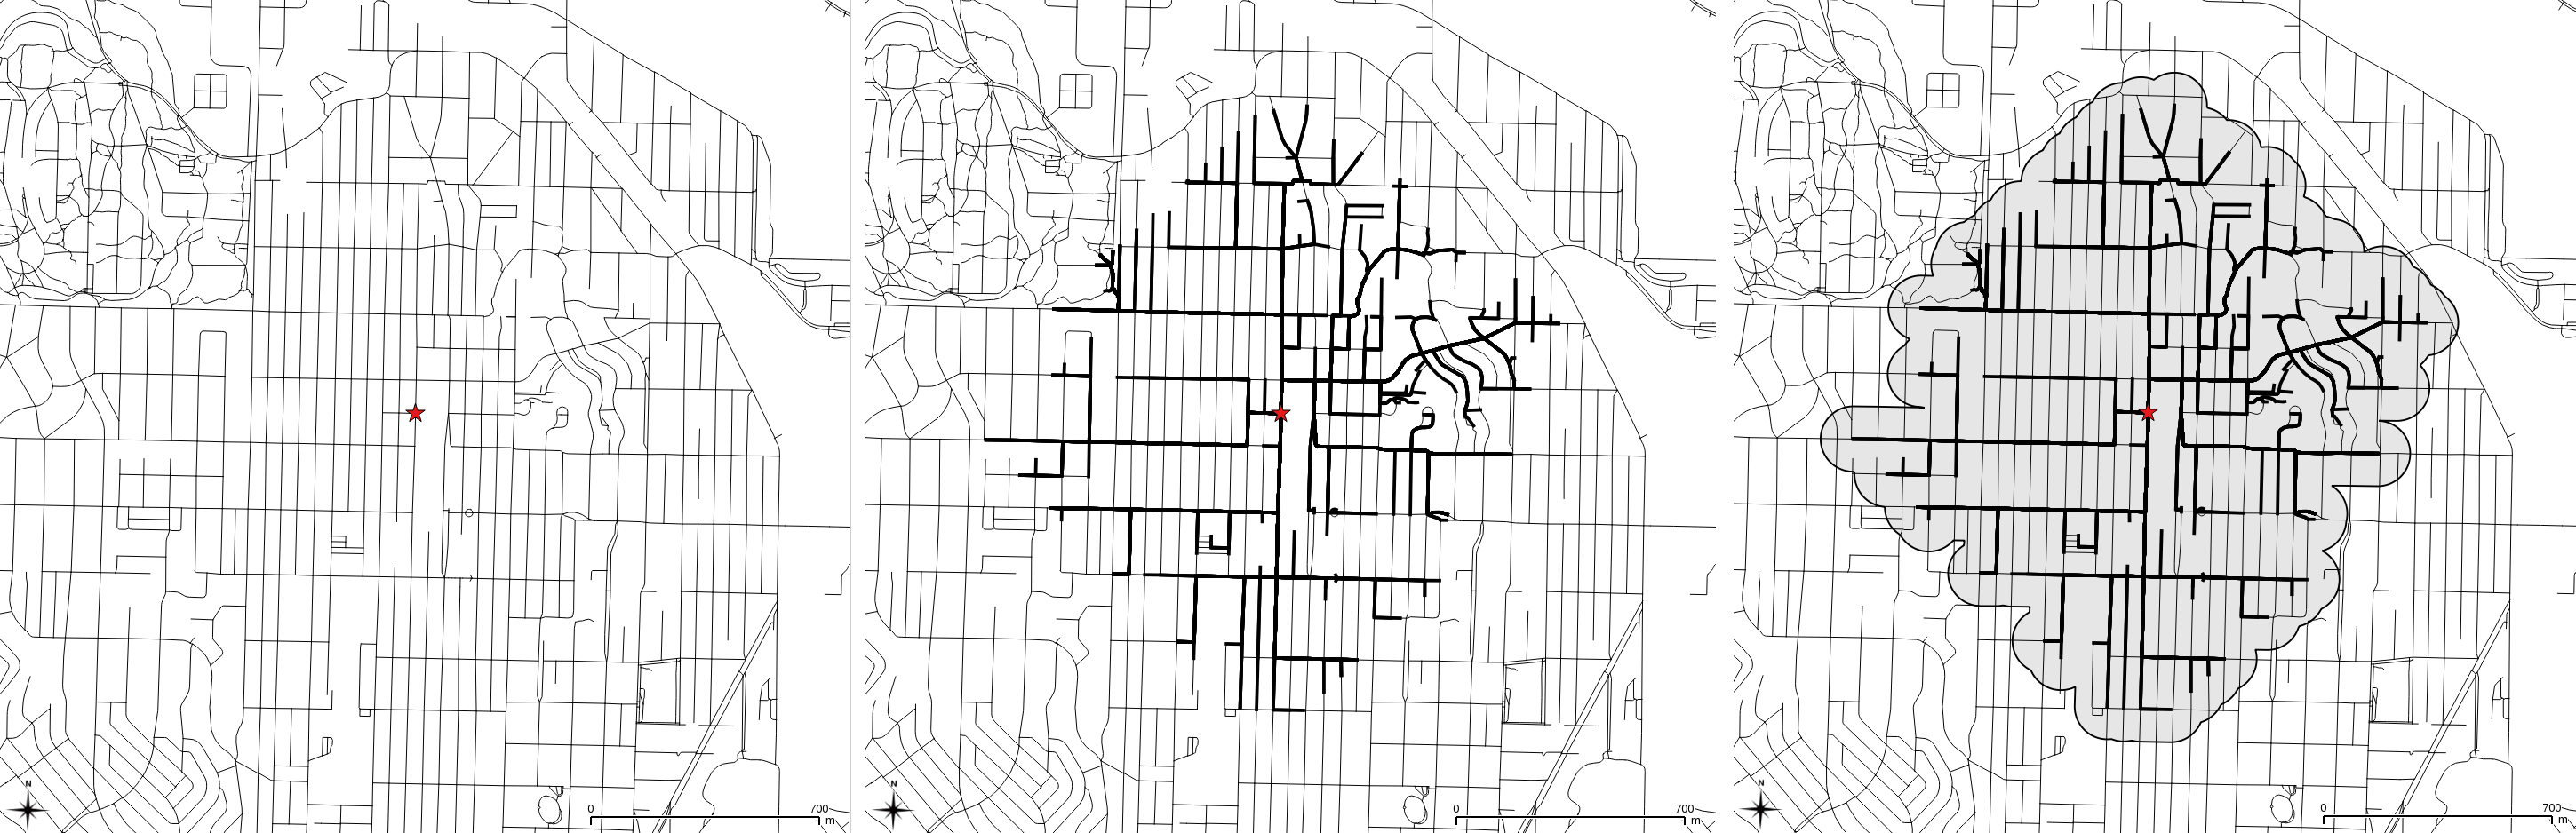
\includegraphics[width=\textwidth]{./figs/sausage-steps}
  \caption{The three primary steps in creating a
    sausage buffer. Left: an origin is selected. Center: the portions
    of the network reachable within a given distance threshold (here,
    1km) are identified. Right: lines are buffered and dissolved.
\textcolor{red}{LET'S MAKE THE POINT OF ORIGIN, NORTH ARROW, AND SCALE BAR MORE PROMINENT}
}
	\label{fig:sausage-steps}
\end{figure}

%\subsection*{Data sources and network import}
To create the routable network required for generating the buffers, we
imported the Washington State portion of the Open Street Map (OSM) (\copyright\ OpenStreetMap contributors)
into PostGIS / pgRouting using the open source osm2pgrouting
utility. \textcolor{red}{Did we use GeoFabrik? If so we should describe.} Because much of the work in measuring built environment exposures deals with pedestrian travel, we
excluded highway facilities, which often do not allow for pedestrian
access. The osm2pgrouting import strategy yielded two primary
benefits. First, osm2pgrouting facilitates reproducible data
importation through the use of an XML-based configuration file, which 
allows facility exclusions to be carried out consistently, such as our exclusion of highways as non-traversible for
pedestrians. Secondly, osm2pgrouting
preserves the topology of the OSM network, rather than relying on
topology created from the data set's simple vector geometry. Maintaining network topology is important for enforcing physical constraints to traversability such as over/underpasses or bridges.

%\subsection*{Generation of buffers}

% Creation of buffer code in database
% Random sample of 200 vertices as points to construct buffers around
% Define sausage buffering procedure in PLSQL
% Construct 1000m buffer (net dist), 100m (arc dist)
% Rounded versus squared ends
We implemented the sausage buffering algorithm in PL/PgSQL, which provides basic SQL functionality as well as procedural characteristics such as control structures and complex computations, with functions saved as stored procedures within the database. We created two functions; the first generates a
sausage buffer around a single point of origin, and the second uses
the first function to generate sausage buffers around an arbitrary
number of points.

Because a point of origin may not be located precisely on the network,
the sausage buffering function begins by identifying and `snapping' to the
vertex in the network nearest to the identified point of origin. To limit the
required number of distance calculations required, the function then
identifies vertices within a circular buffer with radius equal to the
chosen network distance threshold, which represents the maximum
possible distance one could travel on the network in any
direction. We then generate the route to each vertex within this
circular buffer. Because the network distance from the origin to any given vertex could exceed the threshold, we truncated each route using the threshold distance.\footnote{We
  believe this approach to be computationally inefficient, however
  necessary due to the lack of a built-in service area function in
  pgRouting. Our hope is that future versions of pgRouting will
  include service area analysis, thus simplifying and speeding up
  creation of these buffers.} The resulting set of lines are then
buffered according to the buffer radius, and the resulting polygons
are dissolved into a single geometry.

The PL/PgSQL implementation was used to generate buffers originating from 200 points, which were randomly selected from the road data set's network vertices to ensure that they were not located in
roadless areas of the state. Then, in order to compare buffers
created using the PostGIS implementation with ArcGIS-generated buffers, we exported the origin points and OSM network data as shapefiles and followed the protocols described in
\textcite{Forsyth2012proto}, but using rounded buffer ends as described in \textcite{Forsyth2014sausage}. 

Finally, we made two comparisons between the two sets of
buffers. First to assess whether differences in
the planimetric area between these two groups were statistically significant, we
used a Bayesian procedure somewhat analogous to a t-test called BEST
\autocite{Kruschke2014,Kruschke2013}. \textcolor{red}{Why this method instead of a t-test?} Second, to assess the possibility of
spatial misalignment between similarly sized buffers, we computed the
symmetric difference of the two sets of sausage buffers and then
calculated the area of the non-overlapping regions.


\section*{Results}
Overall, the differences between the PostGIS and ArcGIS generated buffers were quite low. Figure
\ref{fig:area_dens} shows the distribution of areas of these two sets of
buffers. Both exhibit the same bimodal shape, with greater
differences observed among smaller buffers. Although the PostGIS-generated buffers were slightly smaller, the mean difference's 95\% confidence interval was -0.23 to 0.04, indicating no significant difference in size using the two methods.

\begin{figure}[h!]
  \centering
  \includegraphics[width=0.65\textwidth]{../results/area_dens}
  \caption{Density plot showing the distributions PostGIS- and
    ArcGIS-generated sausage buffers across the range of sizes.}
  \label{fig:area_dens}
\end{figure}

The symmetric differences between the two sets of
buffers were small (figure \ref{fig:symdiff_dens}), \textcolor{red}{with X being less than Y}. \textcolor{cyan}{Can we add some numbers about the relative size of the differences to the size of the buffers?}. Figure \ref{fig:symmetric_differences} illustrates
three scenarios including the best, typical (closest to the median),
and worst cases with respect to these symmetric differences. In the
best case, the buffers encompassing a very small, isolated
pedestrian facility are practically identical. In the more typical
case, slight differences are visible upon close inspection. Finally,
in the worst case, which was located in a remote portion of Central
Washingtion, the buffers are very different, with
the PostGIS buffer being only a subset of the larger ArcGIS-generated buffer.

\begin{figure}[h!]
  \centering
  \includegraphics[width=0.65\textwidth]{../results/symdiff_dens}
  \caption{Density plot showing the distribution of symmetric
    differences between PostGIS- and ArcGIS-generated sausage buffers.}
  \label{fig:symdiff_dens}
\end{figure}

\begin{figure}[h!]
  \centering
  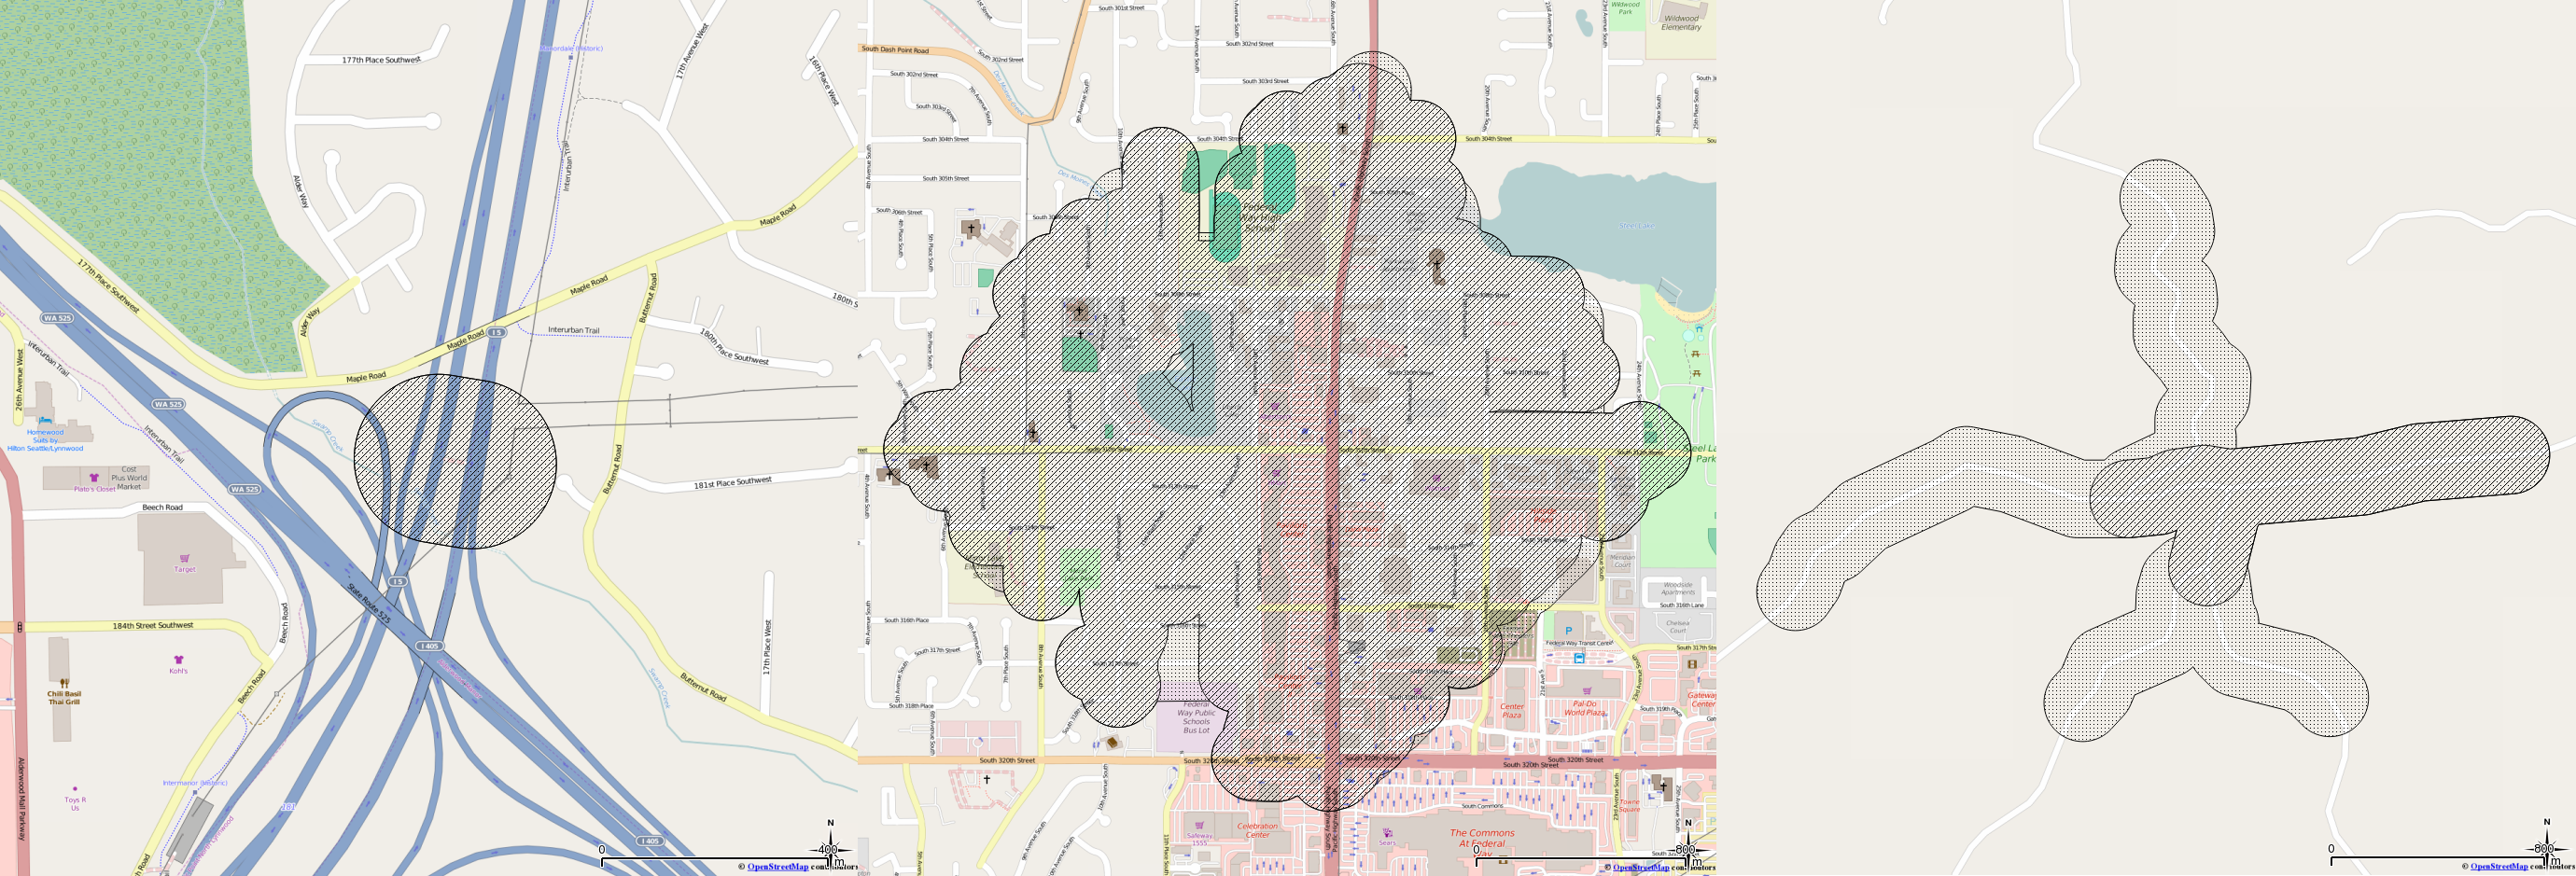
\includegraphics[width=\textwidth]{./figs/symmetric-differences}
  \caption{Three buffers illustrating a range of symmetric
    differences. Left: buffer with smallest difference. Center:
    buffer with difference nearest the median. Right: buffer with largest
    symmetric difference. PostGIS buffered regions are denoted by
    diagonal crosshatching, while ArcGIS buffered regions are
    dot-shaded. \textcolor{red}{Separate these images from each other with whitespace. Subfig or some such. Also can we need a better polygon fill that shows up at a readable size/scale.}}
  \label{fig:symmetric_differences}
\end{figure}

\section*{Discussion}
This study presented a new method for generating sausage buffers using free and open source GIS software, and compared the results of this method to those of an existing method that relies on the leading proprietary GIS application, ArcGIS. 

There were measurable, but not signiticant differences between buffers generated using the two methods. The primary source of differences between the PostGIS
and ArcGIS generated buffers is \textcolor{red}{likely} the result of topological differences
and errors in the network dataset. Osm2pgrouting imports OSM data into PostGIS while preserving network topology. Calculations performed with
PostGIS / pgRouting will properly handle not readily apparent discontinuities,
such as the aforementioned cases of over/underpasses. The network used for creation of buffers in ArcGIS, on the other hand,
was exported as a shapefile from PostGIS. Because shapefiles do not preserve topology,
ArcGIS is forced to infer topology from simple ``spaghetti'' geometry. Thus, in the 
situation where a bridge crosses over another roadway, the
reconstructed network may erroneously connect between the bridge and
the road below. \textcolor{red}{Can we verify this?} In that case, the PostGIS
buffer would be smaller than the ArcGIS buffer, due to the greater, but erroneous 
connectivity in the ArcGIS network. While the mean difference in area
between our two sets of buffers was not statisitcally significant, the observed differences in our sample are consistent with the
logic that the more connected, inferred network topology would yield
larger buffers. \textcolor{red}{OK, sorry to ask, but we really should export back from shapefile to PostGIS as spaghetti for at least one of the bad cases of difference to test whether that was indeed the case. Or examine the roads in that worst case to verify that was happening. Then we needn't rely on a logical argument but can point directly to the cause.}

\textcolor{red}{I don't think we need this.}\st{Our worst case buffer pair suggests an an extreme version of this size
bias with respect to network topology---namely that potential
topological errors in the Open Street Maps data could be corrected
when imported into ArcGIS via a shapefile. These two buffers are
located in a remote portion of Central Washington, where we might
expect network topology errors to go uncorrected, in this instance
resulting in a false discontinuity. In such instances, the PostGIS
buffer would again be smaller than the ArcGIS buffer.} Finally, while
most of the PostGIS-generated buffers were smaller, about 15 percent
were larger than their ArcGIS-generated cognate, suggesting that
inferred topologies may not always be more connected than the topology
present in the OSM data.

\section*{Conclusions}
This paper set out to validate, in a fully reproducible way, the
sausage buffer approach to creating network-based travel catchment
areas. We accomplished this by developing procedures using the
PostgreSQL relational database and its PostGIS and pgRouting
extensions. 

In addition to establishing a reproducible method for creating sausage
buffers, the buffers created using PostGIS and ArcGIS 
are generally comparable. Differences between sausage buffers created in the two
programs are more likely due to differences in how network
datasets are constructed, than to differences in the underpinnings of how the buffers are
computed.

PostgreSQL, PostGIS, and pgRouting provide
suitable analytics and offer important benefits for several purposes.
With automated analyses that are less subject to human error, the sausage buffering procedures presented here achieve a higher
standard of reproducibility than the previously published research. In addition
to our procedures being fully automated through computer code, the
free and open source nature of PostgreSQL, PostGIS, and pgRouting
confer further benefits to reproducibility. Whereas the underlying algorithms used in ArcGIS's Network Analyst are not known outside of Esri,
all of pgRouting's distance calculations and logic can be scrutinized
directly in the source code. Indeed, had the service area calculations in ArcGIS been
fully transparent in this manner, \citeauthor{Forsyth2014sausage} may
not have had cause to develop sausage buffers in the first place.



\printbibliography


\end{document}
